\section{Experiment}
	\begin{figure}[htbp]
	\centering
	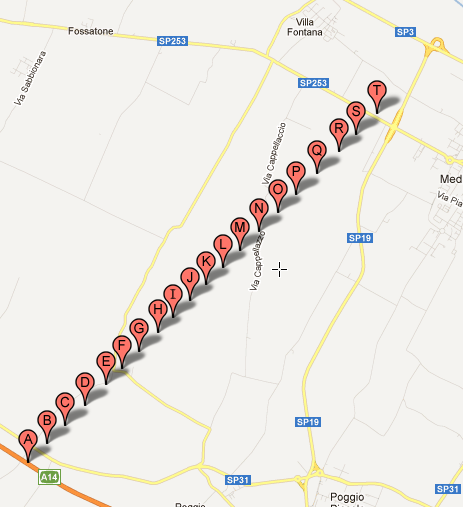
\includegraphics[width=3.4in]{imgs/punti_mappa.png}
	\caption{Fake positions used for the experiment}
	\label{fig:positions_experiment}
	\end{figure}

To try out our testbed applications, we implemented Fast Broadcast algorithm both for Android application and Desktop application. Simulation used a set of fake position distributed on a straight line, each at a random distance between $275$ and $325$ meters from the following. In figure \ref{fig:positions_experiment} a graphical representation can be seen. They covers approximately $8$ kilometers.

\subsubsection{Android application}
To test our Android application we used three Android devices. We performed 10 executions of Fast Broadcast algorithm with the following settings:

\begin{center}
\begin{tabular}{|m{0.22\textwidth}|m{0.12\textwidth}|}
	\hline	
	\ttt{SLOT SIZE} 			& 250 ms \\
	\hline
	\ttt{CW MIN}				& 5\\
	\hline
	\ttt{CW MAX}				& 10\\
	\hline
	\ttt{ACTUAL RANGE}			& 1000 m\\
	\hline
	\ttt{DEFAULT RANGE}			& 300 m\\
	\hline
	\ttt{HELLO MESSAGE TURN}	& 500 ms\\
	\hline
\end{tabular}
\end{center}

%\begin{itemize}
%	\item \ttt{SLOT SIZE 			= 250ms}
%	\item \ttt{CW MIN 				= 5} 
%	\item \ttt{CW MAX 				= 10}
%	\item \ttt{ACTUAL RANGE 		= 1000 m}
%	\item \ttt{DEFAULT RANGE		= 300 m}
%	\item \ttt{HELLO MESSAGE TURN	= 500 ms}
%\end{itemize}

%We first tried an execution wothout range estimation, then with range estimation phase. In the second case, the average amount of time waitd on the contention window by each device resulted to be smaller, and so the contention window size. However, due to the overhead introduced by Hello message exchanging and processing, a solution with static range performs a much faster message propagation.
%In both cases, the overhead introduced by TCP traffic doesn't let the algorithm beahave properly, resulting in some cases in simultaneous message forwarding by different devices.
Slot size was choosen to be $250ms$ to be great enought to reduce simultaneous retransmission of different devices; in fact, due to TCP overhead we noticed that sometimes message did not arrive in time to avoid useless message forwarding. We tried to use UDP protocol to provide a much faster message transmission, but the packet error was too big to obtain a complete simulation. We decided to use this transport protocolo to exchange Hello message, to relieve the TCP server from the traffic generated from this messages.

% UDP EXPERIMENT
%The transport protocol we choose to send out Alert messages was UDP, this to reduce the protocol stack overhead (with TCP was estimated to be $\geq250$ms), speeding up the execution and let us set more realistic parameters values. This was achieved adding a filter to the transport manager at application startup. Hello messages were exchanged using TCP protocol, to reduce the traffic the UDP server thread had to manage.
Execution results are shown in table \ref{tab:Android_res}. Simulation duration, Time waited on contention window and contention window size are the average of the values measured in each device. As we can see, the time needed to carry the Alert message to the last position is quite big, and this is mainly due to the size of the slot and to TCP overhead. The number of Hops in some executions, is equals to the theoretical optimum (With this settings and three devices, optimal hop number is 15). 

\begin{table}
% increase table row spacing, adjust to taste
%\renewcommand{\arraystretch}{1}
% if using array.sty, it might be a good idea to tweak the value of
%\extrarowheight as needed to properly center the text within the cells
\caption{Fast Broadcast simulation results}
\label{tab:Android_res}
\centering
% Some packages, such as MDW tools, offer better commands for making tables
% than the plain LaTeX2e tabular which is used here.
\begin{tabular}{|m{0.06\textwidth}|m{0.08\textwidth}|m{0.08\textwidth}|m{0.08\textwidth}|m{0.07\textwidth}|}
\hline
Execution & Total \newline Time (sec) & Average waited time (ms) & Average Contention Window size & Hops \newline number \\
\hline
1 & 17,0187 & 626,667 & 5,67 & 19 \\
\hline
2 & 15,1167 & 581	  & 5,33 & 15 \\
\hline
3 & 22,0833 & 585,333 & 5,33 & 15 \\
\hline
4 & 16,2190 & 573	  & 5,33 & 19 \\
\hline
5 & 23,3897 & 644,333 & 6	 & 20 \\
\hline
6 & 22,2300 & 639,667 & 5	 & 18 \\
\hline
7 & 15,5160 & 518	  & 5,33 & 20 \\
\hline
8 & 15,5780 & 747,333 & 6	 & 16 \\
\hline
9 & 15,6140 & 606     & 6	 & 15 \\
\hline
10 & 18,997 & 745,667 & 5,67 & 17 \\
\hline
\end{tabular}
\end{table}  
